\documentclass[12pt]{article}
\usepackage{listings}
\usepackage{color}
\usepackage{float}
\usepackage{graphicx}

\definecolor{mygreen}{rgb}{0,0.6,0}
\definecolor{mygray}{rgb}{0.5,0.5,0.5}
\definecolor{mymauve}{rgb}{0.58,0,0.82}

\lstset{ %
	xleftmargin=2em,
	backgroundcolor=\color{white},   % choose the background color; you must add \usepackage{color} or \usepackage{xcolor}
	basicstyle=\small,%\footnotesize,        % the size of the fonts that are used for the code
	breakatwhitespace=false,         % sets if automatic breaks should only happen at whitespace
	breaklines=false,                 % sets automatic line breaking
	captionpos=b,                    % sets the caption-position to bottom
	commentstyle=\color{mygreen},    % comment style
	deletekeywords={...},            % if you want to delete keywords from the given language
	escapeinside={\%*}{*)},          % if you want to add LaTeX within your code
	extendedchars=true,              % lets you use non-ASCII characters; for 8-bits encodings only, does not work with UTF-8
	%	frame=single,                    % adds a frame around the code
	keepspaces=true,                 % keeps spaces in text, useful for keeping indentation of code (possibly needs columns=flexible)
	keywordstyle=\color{blue},       % keyword style
	language=VHDL, % the language of the code
	morekeywords={*,...},            % if you want to add more keywords to the set
	numbers=left,                    % where to put the line-numbers; possible values are (none, left, right)
	numbersep=5pt,                   % how far the line-numbers are from the code
	numberstyle=\small\color{mygray}, % the style that is used for the line-numbers
	rulecolor=\color{black},         % if not set, the frame-color may be changed on line-breaks within not-black text (e.g. comments (green here))
	showspaces=false,                % show spaces everywhere adding particular underscores; it overrides 'showstringspaces'
	showstringspaces=false,          % underline spaces within strings only
	showtabs=false,                  % show tabs within strings adding particular underscores
	stepnumber=1,                    % step between two line-numbers. If it's 1, each line will be numbered
	stringstyle=\color{mymauve},     % string literal style
	tabsize=2                  % sets default tabsize to 2 spac                  % show the filename of files included with \lstinputlisting; also try caption instead of title
}
%opening
\title{Project 1: Designing a 16-bit Register File}
\author{Adam Sumner \\ ECE 485}
\date{October 6\textsuperscript{th}, 2015}

\begin{document}

\maketitle

\section{Introduction}
The purpose of this project is to implement an 8 by 16-bit register file in the VHDL hardware description language. The register file should be able to output the contents of two registers, and it should be able to write into one of the registers at the positive edge of the clock if an external ``registerWrite" signal is set to 1.
\section{Design}
\subsection{Architecture}
To enable the specific functionality requested in the project, the file needs to have certain attributes. In order to output two register values at the same time, it must have two outputs of 16 bits each: \texttt{outReg1} and \texttt{outReg2}. This solves how the file will display register values, but since there are 8 registers total, functionality must be included to select which two registers to show. This is why \texttt{inReg1} and \texttt{inReg2} are a necessity to include in the architecture. They are both three bit inputs to select which register number (in binary) to display. The schematic for this is shown in Figure \ref{fig:read}. Now that an architecture has been built to select and output two register's content, an architecture for writing contents into a register must also be included. Similar to the architecture for reading registers, a 16-bit data field for writing data into a register (\texttt{writeData}) and a three bit input (\texttt{writeReg}) is used to select which register to write the data to. The schematic for this implementation is shown in Figure \ref{fig:write}. With these both in place, our schematic now at its core looks like that of Figure \ref{fig:register_file}. With the core architecture implemented, a \texttt{clk} and \texttt{writeEnable} must be included so that both a signal can be set to enable the write process, and also so that writing will only happen at the positive edge of the clk. All of the discussed attributes and architectures are declared in the entity section of Section \ref{sec:code}.
\vspace{2cm}
\begin{figure}[H]
\centering
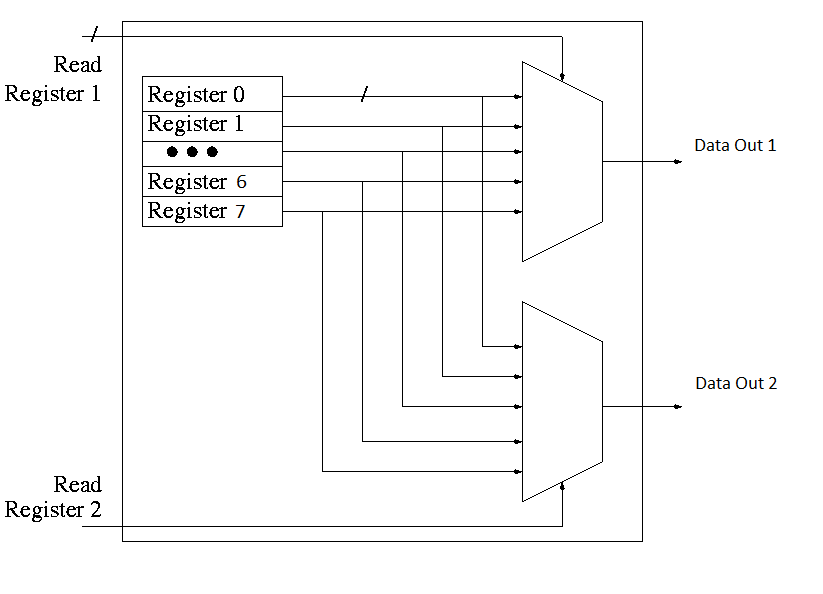
\includegraphics[width=\linewidth]{read-ports}
\caption{Schematic for Reading Two Registers}
\label{fig:read}
\end{figure}


\begin{figure}[H]
\centering
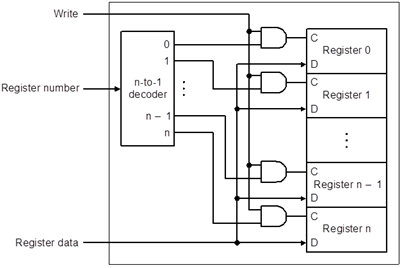
\includegraphics[width=0.8\linewidth]{write}
\caption{Schematic for n-register Write Functionality}
\label{fig:write}
\end{figure}

\begin{figure}[H]
\centering
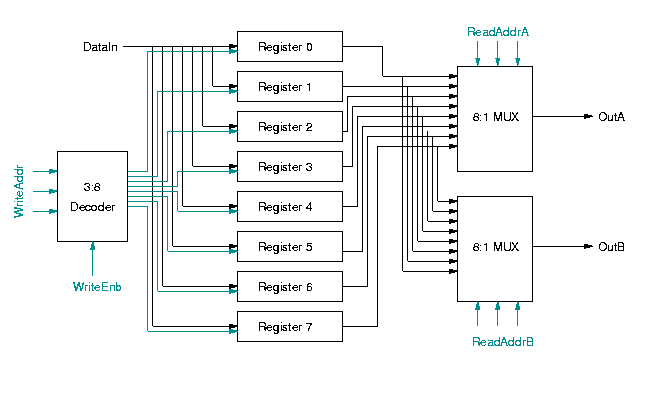
\includegraphics[width=\linewidth]{register_file}
\caption{High Level Design Schematic}
\label{fig:register_file}
\end{figure}

\subsection{Behavior}
The behavioral section of the code in Section \ref{sec:code} is pretty straightforward. An array of 8 16-bit data vectors is declared, and a process is defined for the \texttt{clk} signal. If the \texttt{clk} is at its rising edge, then the data from the selected two registers is put into the respective output field. If \texttt{writeEnable} is also 1 on the rising edge of \texttt{clk}, the the data held in \texttt{writeData} is put into the selected register determined from \texttt{writeReg}. Note that registers are only read on the rising edge of the \texttt{clk}. This was decided to make the design process simple and to define a standard that events will only execute during the start of a \texttt{clk} cycle.
\subsection{Code}\label{sec:code}
\lstset{language=VHDL}
\lstinputlisting{../register.vhd}
\begin{lstlisting}

\end{lstlisting}
\section{Simulation Results}
This section will walk through a test simulation to ensure the functionality of the register file is correct. All registers will start with value $0000000000000000_2$. Value $1000000000000000_2$ will be written into register 2 and value $0000000000000001_2$ will be written into register 7. These registers will then be read. A clock cycle of 10 ns will be used. The start of the simulation is shown in Figure \ref{fig:sim-start}.

\begin{figure}[H]
\centering
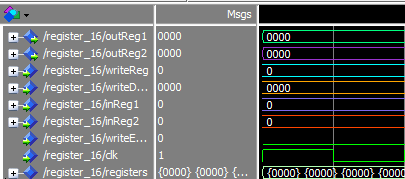
\includegraphics[width=\linewidth]{sim-start}
\caption{Start of Simulation}
\label{fig:sim-start}
\end{figure}

Then the value $1000000000000000_2$ is put into \texttt{writeData}, the value $010_2$ is put into \texttt{writeReg}, and the \texttt{writeEnable} is set. This is shown in Figure \ref{fig:write1}. 

\begin{figure}[H]
\centering
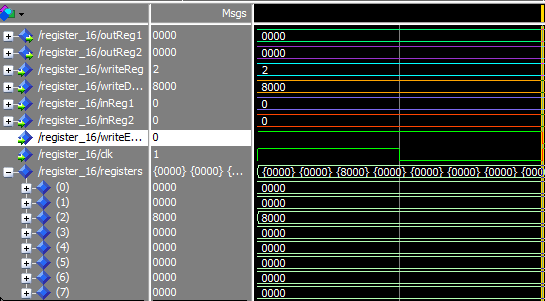
\includegraphics[width=1\linewidth]{write1}
\caption{First Write}
\label{fig:write1}
\end{figure}

Then the value of  $0000000000000001_2$ is put into \texttt{writeData} and the value $111_2$ is put into \texttt{writeReg}. This is shown in Figure \ref{fig:write2}.

\begin{figure}[H]
\centering
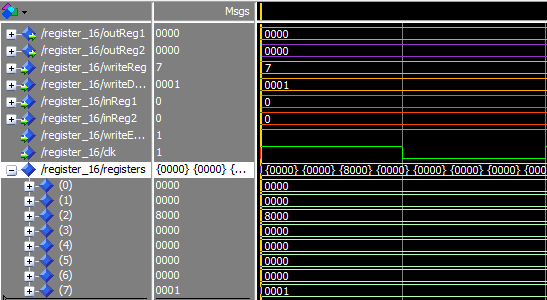
\includegraphics[width=1\linewidth]{write2}
\caption{Second Write}
\label{fig:write2}
\end{figure}

Now \texttt{writeEnable} is set to 0, \texttt{inReg1} is set to $010_2$ and \texttt{inReg2} is set to $111_2$. This is shown in Figure \ref{fig:sim-read}. 

\begin{figure}[H]
\centering
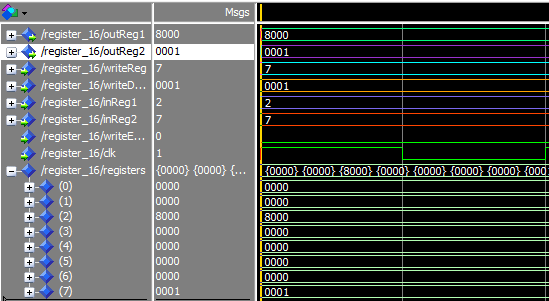
\includegraphics[width=1\linewidth]{sim-read}
\caption{Reading Values from Registers}
\label{fig:sim-read}
\end{figure}

It is clear from the simulation results that the register is behaving as intended.
\section{Conclusion}
The construction of an 8 by 16-bit register file was a success. An architecture and behavior was designed around the register file constraints, and the final product performed as expected. This register file can now be used in further projects.
\end{document}
